\documentclass[titlepage,a4paper,12pt]{book}

\usepackage[utf8]{inputenc}
\usepackage[catalan]{babel}
\usepackage{graphicx}
\usepackage{verbatim}
\usepackage{marvosym}
\usepackage{amssymb, amsmath} 
\usepackage{listings}
\usepackage{textcomp}
\usepackage[]{color}

%\lstset{
	%language=C++,
	%keywordstyle=\bfseries\ttfamily\color[rgb]{0,0,1},
	%identifierstyle=\ttfamily,
	%commentstyle=\color[rgb]{0.133,0.545,0.133},
	%stringstyle=\ttfamily\color[rgb]{0.627,0.126,0.941},
	%showstringspaces=false,
	%basicstyle=\small,
	%numberstyle=\footnotesize,
	%numbers=left,
	%stepnumber=1,
	%numbersep=10pt,
	%tabsize=2,
	%breaklines=true,
	%prebreak = \raisebox{0ex}[0ex][0ex]{\ensuremath{\hookleftarrow}},
	%breakatwhitespace=false,
	%aboveskip={1.5\baselineskip},
  %columns=fixed,
  %upquote=true,
  %extendedchars=true,
%% frame=single,
%% backgroundcolor=\color{lbcolor},
%}

\begin{document}
\tableofcontents  %%Index
\section{Objectius} % (fold)
\label{sec:Objectius}
Aquest projecte anomenat \texttt{Pholus}, ha estat desenvolupat per a equilibrar
(ponderar) pesos dels diferents indicadors de semblança entre molècules, per a
veure quins són més rellevants en discriminar les que poden tenir una activitat
més òptima en front una diana. 

Es tracta d'un algoritme evolutiu relativament senzill pel que fa al propi algoritme, però més
complex pel referent a les condicions externes que s'imposen per la natura, i que ens obliguen a
posar condicions i limitacions al Algoritme Evolutiu (als Algoritmes Evolutius
no els agraden les limitacions).

Pholus forma part de la nova tecnologia desenvolupada per Intelligent Pharma, anomenada HELIOS, que
serveix per identificar,a partir d'un compost de referència prèviament donat, nous compostos amb
propietats estructurals completament diferents que imiten el comportament d'aquest compost de
referència. Per exemple, si el compost de referència ja és conegut (per exemple, un extret d'un
producte natural o d'una patent), HELIOS pot trobar compostos no  vinculats estructuralmnt que
reprodueixin les seves propietats psico-químiques tridimensionals; per tant, aquests compostos
tindran les mateixes característiques biològiques però amb diferent estructura mol·lecular. A
aquesta búsqueda se l'anomena "Scaffold hopping" (búsqueda entre diferents famílies químiques).

La tècnica utilitzada és el Virtual Screening(VS), que normalment s'utilitza per descobrir noves
famílies químiques en relació a una activitat biològica desitjada. El VS té mètodes que es basen en
l'estructura dels compostos i d'altres que no. Com hem dit, HELIOS té com a objectiu identificar
nous compostos que no són anàlegs estructuralment, però sí biològicament. 

HELIOS es basa en la superposició de camps mol·leculars entre qualsevol compost i un lligand de
referència. Però HELIOS, no només considera la superposició generada per càrregues formals, sinó
també altres tipus relacionades amb el comportament dinàmic; així, es fan diferents superposicions
entre parells de mol·lècules es duen a terme a la vegada. 
L'alineament de camps mol·leculars va ser descrit durant els anys noranta, però no s'ha dut a terme
fins aquesta dècada degut a que l'alineament mol·lecular flexible és un problema impossible de
resoldre sense les eines de supercomputació. Fins els últims anys, el Virtual Screening basat en els
lligams s'ha basat en metodologies per buscar semblances moleculars com l'estructura, farmacòfor,
etc. 

HELIOS utilitza alineaments de camps moleculars flexibles per identificar compostos que s'assemblin
a un compost de referència. L'alineament molecular e duu a terme mitjançant tècniques de "cloud
computing", la qual permet fer-ho en pocs dies. Els compostos amb els quals es fa l'alineament es
treuen d'una base de dades que pot variar segons l'objectiu de la búsqueda. 

Els camps moleculars són discretitzats dins d'una caixa en forma de grid de punts. Idealment, la
caixa hauria de ser suficientment gran per introduir-hi tots els lligans de la base de dades en una
conformació extesa. De la mateixa manera la capsa ha d'incloure aquells punts al voltant de les
molècules que tenen valors significatius. Diferents representacions dels camps moleculars, que donen
diferent informació sobre la densitat electrònica, són construits amb sondes atòmiques. Una sonda
atòmica és una partícula amb característiques químiques particulars que s'assemblen a propietats
atòmiques en ambients electrònics particulars. 

Les 22 sondes atòmiques que són implementades en HELIOS són les que  es veuen a la taula \ref{table:maps} 

\begin{table}
\centering
\begin{tabular}{|ccc|}
\hline
aromatic carbon &aliphatic carbon&non-hydrogen bonding sulfur\\
non-hydrogen bonding phosphor&phosphor&non-hydrogen bonding nitrogen\\
hydrogen donor&oxygen acceptor&nitrogen acceptor\\
sulfur acceptor&spherical nitrogen acceptor&spherical oxygen acceptor\\
fluorine&chlorine&bromine\\
iodine&iron&manganese\\
calcium&magnesium&zinc\\
positive charge&& \\
\hline
\end{tabular}
\caption{The 22 atom probes implemented in HELIOS.}
\label{table:maps}
\end{table}

El camp molecular definit per una sonda en un punt donat és calculat amb la
següent equació % XXX : TREURE-HO, no?

L'alineament múltiple de camps moleculars flexibles és una taxa complexa que requereix de tècniques i recursos computacionals avançats. El procés implementat per HELIOS fixa el camp molecular del compost de referència i utilitza algoritmes evolutius en un sistems de "cloud-computing" per duu a terme l'alineament flexible múltiple dels camps moleculars de cadascún dels diferents compostos que hi ha dins la base de dades.

Amb això obtenim per a cada mol·lècula de la base de dades 22 vectors on hi ha els valors per cadascún dels punts ordenats del grid de les 22 sondes moleculars. A partir d'aquí hem de trobar alguna manera d'evaluar la similitud entre mol·lècules.

Com es mostrarà en les següents seccions, hi ha una part important de feina
realitzada en la preparació de les dades, i en la corresponent validació dels
resultats a part del propi algorisme evolutiu.

% section Objectius (end)

\section{Context Químic} % (fold)
\label{sec:Context Quimic}
Tanimotos, conformacions, y tal 

El problema al que ens enfrontem és el de, donat un \texttt{receptor} i un conjunt de %glossari
\texttt{lligands}, deduir quins són els factors que fan que la unió sigui millor
o pitjor.  Els factors que intervenen en aquesta unió són molts, però a nivell
pràctic, utilitzem ``només'' 22 indicadors de potencial, que són els que podem quantificar amb
facilitat, i que hem cregut que tenen més rellevància en aquest procés.

Aquests indicadors són:

\begin{table}
\centering
\begin{tabular}{|ccc|}
\hline
aromatic carbon &aliphatic carbon&non-hydrogen bonding sulfur\\
non-hydrogen bonding phosphor&phosphor&non-hydrogen bonding nitrogen\\
hydrogen donor&oxygen acceptor&nitrogen acceptor\\
sulfur acceptor&spherical nitrogen acceptor&spherical oxygen acceptor\\
fluorine&chlorine&bromine\\
iodine&iron&manganese\\
calcium&magnesium&zinc\\
positive charge&& \\
\hline
\end{tabular}
\caption{The 22 atom probes implemented in HELIOS.}
\label{table:maps}
\end{table}

Per tal que una unió entre lligand i receptor sigui bona, les energies
dissipades s'han de minimitzar, mostrant així que entre les dues molècules es
neutralitzen.  Si la energia és alta, fa que la estructura final (lligand +
receptor) sigui poc estable i fàcilment trencada, ja que les dues parts, poden
trobar alguna altra formació on ``es troben més còmodes'' i desfan la unió que
tenien.

% XAVISTART

Per començar, hem d'imaginar una molècula com un graf en un espai de tres
dimensions, on els nodes són els àtoms, i les arestes són enllaços.  En general,
semblança $S_{A,B}$ entre dos objectes és estimada pel nombre d'elements iguals
que tenen. Els objectes que són iguals, haurien de tenir la màxima puntuació.
Per tant, una expressió de la semblança sería en termes de la teoria de
conjunts, la intersecció $(A\cap B)$ que en lògica seria l'operador $AND$. La
dissimilitud $D_{A,b}$ és estimada pel nombre d'elements diferents que tenen.
Els objectes idèntics obtindrien la mínima puntuació. Anàlogament a la
similitud, parlant en termes de teoria de conjunts, la dissimilitud es
calcularia posant amb la unió $(A\cup B)$ o el que seria el mateix amb
l'operador lògic $OR$. El denominador serà simplement un normalitzador per tenir
l'índex entre 0 i 1. 

El concepte de semblança normalment s'utilitza per referir-se tan a la semblança
com a la diferència, ja que es suposa que si dos objectes són semblants és
perquè no són diferents. En matemàtiques i estadística s'utilitzen els conceptes
de semblança, proximitat i distància per referir-se al mateix, però en química,
similitut i dissimilitut poden portar a diferents resultats. Per exemple,
considerem dues seqüències de caràcters, F1 i F2, cadascuna té conjunts de 407
caràcters, 402 dels quals són comuns entre ells. F3 i F4, cadascuna té un
conjunt de 5 caràcters, dels quals cap d'ells és comú. En els dos casos la
distància Euclídia és $10 \over 1024$  o $0.0098$ quan és evident que les dues
primeres són més semblants entre elles que la segona parella.

%Continues vs Discretes? bedroc.tex pag 11

Mètriques per a mesurar els potencials i les diferències (o semblances) entre
ells n'hi ha moltes, unes funcionen millor per a dades qualitatives, altres per
a quantitatives, i n'hi ha que fins i tot utilitzen la falta d'informació per a
establir similituds.  Això últim, en el nostre context no ens interessa tant com
tenir una mesura que ens serveixi per a dades quantitatives, i a ser possible,
acoti els valors entre dos llindars coneguts.

Hem de tenir en compte el cost de calcular les diferències entre molècules, ja
que serà un procés a repetir moltes vegades, i en gran número de molècules, i
hem d'intentar trobar un coeficient que sigui viable de calcular.  Ens hem
decidit per una variació de Tanimoto, acotada entre -1 i +1 que s'explicarà tot
seguit.

%XAVISTOP  XXX

Per a calcular els valors dels 22 potencials de cada lligand, es resten els
potencials de la molècula de referència amb els del lligand.  El format en el
que estàn ambdues molècules, és el mateix, però pot ser que estiguin situades en
un espai diferent respecte el 0 del eix de coordenades (recordem que estan
mapejades en un espai 3D).  Per a ajustar les dues molècules, es passen per un
procés de docking (autodock), que el que fa es ajuntarles de la millor manera que pot
(també utilitza algoritmes genètics per a fer-ho) simulant la seva unió. Una
vegada tenim els dos grafs ``superposats'' de la millor manera, calculem les
diferències entre els potencials d'una i de l'altre estructura en cada punt, i
després podem fer una resta dels valors punt a punt.  Això ho podem fer gràcies
a què hem reduit les dues molècules a ocupar el màxim espai comú, i els
potencials en cada punt $i$ de la matriu de la molècula de referència, pot ser
relacionat i comparat amb el punt $i$ de la matriu d'un lligand.

Després de fer tots els calculs i restes pels 22 diferents tipus de potencials,
podem donar un número de semblança ``total'' per dos molècules i un tipus de
potencial.

Tanimotos. Què cony son? %XXX
\subsubsection{Tanimoto} % (fold)
\label{ssub:Tanimoto}

% subsubsection Tanimoto (end)

\subsubsection{Estereoisomers i conformacions}
\label{ssub:estereoisomers i conformacions}

Una altra particularitat del problema és la varietat de estereoisomers i de
conformacions que pot tenir una molecula donada.  Una molècula, identificada per
un nom i una composició pot tenir diverses maneres de mapejar-se en un espai
tridimensional.

Quan diem que una molècula pot tenir varis estereoisomers, ens referim a que
dues molècules, poden ser simètriques, però no superposables.  Un exemple al que
podem estar més acostumats, per entendre el concepte són les mans.  La mà dreta
i la esquerra, tindrien la mateixa composició, però al ser simètriques una
respecte la altra, fa que no puguem superposarles.

Cada estereoisomer pot tenir diverses conformacions.  Amb això ens referim a què
en la natura, no sempre trobem la molècula amb els mateixos angles entre atoms,
tipus d'enllassos, etc. Per exemple, una molècula pot trobarse en la natura
enrotllada sobre ella mateixa, o bé estirada (és bastant comú trobar aquests
tipus de conformacions).

%XXX Fotos de isomers i conformacions

Quan sabem que una molècula és activa, podem no tan sols buscar la minimització
d'energia (és una feina costosa, i no podem controlar tots els agents externs
presents en l'entorn), sinó que podem, simplement refiar-nos de que sabem
empíricament que la activitat d'un lligand amb un receptor.

%XXX quan tenim molecules actives, no tenim la conf ni isomer, i hem de buscar
%d'entre totes, la millor, i fiarnos que aquella es la bona, per comparar amb
%les que busquem


El que utilitzem és la informació de molecules que sabem que són actives,
i elaborem tot el procediment per a descobrir quines condicions compleixen entre
elles que les pot fer actives.

Així doncs, les dades que tenim com a entrada són simplement els 22 valors per a
cada molecula (isomer X conformació), i una llista de quines d'elles sabem del
cert que presenten activitat contra un receptor donat.  El que volem aconseguir
és doncs, 22 factors, pels que multiplicar els 22 \textbf{tanimotos} i que al
sumar-los, ens donin una ordenació de les molècules, situant les actives en
les primeres posicions (un index de activitat?).

% XXX Formula

Inicialment, hem provat la intuició química, per decidir quin tipus de
indicadors són els més rellevants, i ajudats amb eines estadístiques, hem
aconseguit trobar unes ponderacions que situen la majoria de molecules actives
en les primeres posicions, però el procés és manual, i no assegura ni la
ordenació actives/inactives, ni la propia ordenació de les actives al principi
de la llista (no totes les actives són ``igual'' d'actives).
% section Context Químic (end)

\section{Procediment informàtic} % (fold)
\label{sec:Procediment informatic}

Desde el punt de vista estrictament informàtic, el problema es pot descriure de
la següent manera:

Tenim una entrada de dades d'un conjunt de molècules (amb un identificador
únic) amb els seus 22 valors associats a cadascuna de les sondes escollides, i una
llista amb les molècules actives (els ids).

Utilitzem un algoritme evolutiu, per trobar els 22 valors (ponderacions) als que
multiplicar cadascun dels potencials, que fan que obtinguem una ordenació de les
molècules que classifica les actives al principi.

El procés però, no és tant directe com això, ja que les dades s'han de
pretractar, per a treure molècules errònies, o bé triar quines de les molècules
volem que continuin el procés i quines no (hi ha molècules que son molt similars
entre elles, i no les volem, ja que podrien decantar (bias) l'algoritme genètic cap al
sobreentrenament al seu favor, quan en realitat pertanyen al mateix grup de
molècules.  S'han provat diferents tècniques d'agrupament (clustering), però no ens hem
quedat amb cap , perquè no ens han donat resultats millors amb cap de les
tècniques que s'han usat (K-means, etc) %XXX : Noms de clusteritzacions

Una vegada fet el nucli, la interfície amb l'usuari final també s'ha hagut
de preparar separadament del algoritme genètic, ja que el nostre usuari,
prefereix un entorn amigable (web, GUI, e-mails, excel) abans que entorns més
austers (però configurables i scriptables) com pot ser una simple linia de
comandes.  

% subsubsection subsubsection name (end)
% section inf (end)
\subsection{Interfície} % (fold)
\label{sub:Interficie}

Per a la intefície amb l'usuari, s'ha escollit una interfície web, que executará
l'usuari desde una web corporativa, amb accés restringit i controlat amb
Autenticació.  Això ens porporciona informació de quin usuari executa cadascun
dels càlculs, i així podem personalitzar la presentació, segons preferències de
cadascun.  Utilitzant la web corporativa, ens estalviem haver de gestionar els
permisos que té cada usuari, ja que la interfície que se li presenta, és
adecuada per als seus permisos i les seves tasques a realitzar.

Les dades que entra un usuari són 3 llistes de molècules:

\begin{itemize}
	\item \textbf{Llista d'actives}.  Són les molècules de referència que l'usuari sap
	que tenen activitat positiva davant d'un target concret.
	\item \textbf{Llista d'inactives}.  Molècules que l'usuari sap que són inactives en
	aquest mateix target.
	\item \textbf{Llista de decoys}.  Conjunt de molècules que l'usuari posa ``per
	omplir'', sabent que son inactives també, però amb certes propietats que
	blablabla %XXX 
\end{itemize}

A part de les llistes de molècules, l'usuari també entra els parametres alpha,
RieMax, i els percentatges de molècules amb els que vol provar l'experiment.  Es
deixa la opció de no fer participar totes les molècules en l'experiment deixant 
un conjunt de molècules fora, per després evaluar i validar les dades obtingudes
(l'usuari pot fer manualment 10 fold validation, etc\dots).  Més endevant en 
\ref{sub:sobreentrenament} s'explicarà el sistema de tests i validació.

Per facilitar la usabilitat, el programa proporciona sempre uns paràmetres
estimats per defecte, en funció de les característiques de les llistes que hagi
entrat l'usuari. 
%XXX : Explicar alpha?

% subsection Interfície (end)
\subsection{preparació de dades} % (fold)
\label{sub:preparacio de dades}
Una molècula es pot trobar en la natura en diverses formes.  Les clasificacions
es divideixen en isomers i conformacions.  Una molècula pot tenir diversos
isomers, i cada isomer es pot trobar en  diverses conformacions.

És a dir, que per un nom (o id), en la natura existeixen diverses estructures, que
comparteixen nom, i elements, però poden estar organitzats de forma diferent en
l'espai. Aquestes organitzacions són simètriques en l'espai 3D, donant lloc a
molècules similars, però que en l'espai 3D, no es superposen de la mateixa
forma. (exemple, les mans, que no es poden superposar en 3D tot i ser
simètriques).  Les conformacions, en canvi, són variacions de la posició dels àtoms en l'espai,
però mantenint els enllaços entre àtoms. En les conformacions, el que canvia és
l'obertura en els angles rotables de la molècula.  
Per passar d'un estereoisomer a un altre, s'han de trencar enllaços, i tornar-se
a formar.  En les conformacions no passa això, i es pot passar d'una a una
altra, només canviant els angles dels enllaços i la seva flexibilitat. 

Donat un conjunt de molècules que volem utilitzar, hem de saber quina de les
conformacions triarem per a cada molècula.  Per a fer la \texttt{explosió} de
combinacions, s'utilitza un sofware propietari especific (Corina), que fa la
combinatòria i genera les possibles variacions sobre una molècula donada.
Després de fer aquesta explosió de combinacions, tenim diverses entrades per a
cadascuna de les molècules inicials.  Les molècules que sabem que són actives,
sabem que ho són, però no sabem quina conformació i isomer és el que la fa
activa.  És per això, que en el llistat d'actives, tenim només una entrada per a
cada família de molècules actives, tot i que en la taula de tanimotos, aquesta
molècula estarà representada en diverses entrades. 

Durant la execució del programa, el que fem, és ordenar la llista de tanimotos,
amb molècules ``repetides'', i al moment de fer la puntuació de la llista
ordenada, ens quedem només amb la millor conformació de cada família.

\subsubsection{Procés de preparació} % (fold)
\label{ssub:Proces de preparacio}

Després que l'usuari entri els paràmetres, la web llança una aplicació en Perl,
que fa la preparació de les dades, i és la que llança l'algorisme evolutiu.  El
primer que fa és , recuperar les taules, d'una base de dades (la web emmagatzema
les llistes a una BBDD MySql).

Com s'ha explicat anteriorment, per a fer les validacions, aïllem una part del
conjunt de molècules del experiment per a fer validacions a posteriori, i
assegurar-nos que no hi ha hagut sobreentrenament.

El primer pas que fem és doncs, separar els tres conjunts de molècules, en 3
subgrups, ajustant-nos als paràmetres desitjats per l'usuari.  Per a fer les
validacions, el percentatge de molècules actives e inactives, hauria de
mantenir-se en cadascuna dels tres subgrups. No ens serveix un algoritme que
deixi lloc a la incertesa (encara que en mitja funcioni), com podria ser, treure
números aleatoris entre [0,1) i en funció d'on estigui (separem el segment [0,1)
en tres trossos anteriorment ) colocarlos en un o altre grup, sinó que calculem
el percentatge d'actives respecte al de inactives, i anem omplint els grups fins
a cobrir el llindar.  Això, que pot semblar un detall d'implementació
``despreciable'', no ho és, ja que quan disposem de poques dades (sobretot en
les actives), deixar lloc al atzar pot provocar canvis dràstics (i tràgics) en
els resultats finals.

%Posar implementacions de Agafar els numeros aleatoris

El segon pas és fer l'explosió de combinacions de molècules possibles (isomers i
conformacions).

A un conjunt de molècules, l'hi hem de trobar tots els isomers i les
conformacions diferents en les que es poden trobar a la natura, és per això que
primer, donada una base de dades de molècules diferents, hem de generar totes
les conformacions possibles de cada molècula.  Aquest procés es realitza
mitjançant un programa existent ja (Corina, NO és OpenSource).

Al generar els diferents isomers i conformacions, afegim identificadors a les
molècules, per saber de quina molècula inicial provenien però també saber
exactament quin isomer-conformació és.  Així, si d'una molècula A, generem:

\begin{verbatim}
A_i001_c001
A_i001_c002
A_i001_c003
A_i002_c001
A_i002_c002
A_i002_c003
\dots
\end{verbatim}


Aquí ens sorgeix un possible problema.  Al fer la explosió de combinacions, ens
trobem que les bases de dades, ja no estan balancejades amb els percentatges tal
i com estaven abans, sinó que en funció de les variacions que tinguin les
molècules que han entrat en cada grup (trainning, test i validació), podem
trobar un conjunt molt més poblat del que ens esperariem, i que varii també el
seu percentatge intern de actives/inactives. Per exemple, la molècula A, pot
tenir 6 ``descendents'', i en canvi, la molècula B pot tenir-ne només 2.

Després de consultar amb experts químics, s'ha decidit que això no influiria
negativament en els resultats finals, ja que si una molècula és més versàtil que
una altra, això mateix és un tret propi de la molècula, i està bé que es vegi
potenciada i així, tingui més participació en la llista on pertany.

Una vegada tenim les 6 llistes separades (normalment treballem amb 80\% de
conjunt d'entrenament, un 10\% de test i un 10\% de validació, i per cada una
fem una llista d'actives i una de inactives per a cada grup),  hem de filtrar la
taula d'actives, per tal que no hi hagi els  isomer-conformacions de cada
molècula, sinó que aparegui només una vegada el nom genèric de les molècules
actives.  Això ho fem perquè quan sabem que una molècula és activa, sabem que ho
és la ``família'' de molècules però per una banda, només ho serà en una de les
conformacions i per altra, no tenim informació de quina és aquesta.  És per això
que quan després fem els matchings, els fem només amb la part genèrica de cada
molècula.

%PUNT

% subsubsection Procés de preparació (end)

En aquest punt, ja es disposen de totes les dades tal i com les volem per a
executar l'Algoritme genètic.  El procés intern de l'Algoritme genètic, i els
seus paràmetres en detall s'explicaràn en la secció pertinent ,
\ref{sub:Algoritme genetic}.  En el cas que l'usuari hagi configurat la execució
per a fer-se amb test i validació, la execució només es fa utilitzant com a
dades el conjunt d'entrenament, deixant les taules de testing i validació per a
un procés posterior.

L'algorisme, dóna com a sortida les diferents poblacions que han anat apareixent
al llarg de les diferents generacions.  Així es disposa de dades per a saber com
ha estat el procés evolutiu (per exemple ens permet fer desviacions típiques
sobre les generacions per a saber la convergència) , i ens proporciona armes per
a decidir si podem utilitzar menys generacions per a aconseguir resultats
similars.

Una vegada tenim les ponderacions que han anat apareixent, parsegem aquestes
dades i n'extraiem els millors individuus de cada generació.  Aquests individuus
ens serveixen per divèrses coses:

\begin{itemize}
	\item Poder graficar d'una manera simple la evolució de l'entrenament
	\item Reduir el volum de dades ``utils''.
	\item El millor individu de la última generació serà el que agafarem com a
	resultat final de la aplicació
\end{itemize}

Si l'usuari ha configurat el procés per a utilitzar testing i validació, en
aquest moment, enfrontem les millors ponderacions de cada generació amb les
taules de testing i de validació (per separat).  Aquest procés no implica cap
algorisme genetic, però s'utilitza \textbf{exactament} la mateixa funció que en
l'algorisme genètic (el mateix .h i .cpp).  Això es fa perquè les funcions de
fitness han anat canviat al llarg del temps, afegint petites modificacions sobre
la inicial, i d'aquesta manera, asegurem la consistència entre les dades.

Una vegada tenim els BedRocs que donen cadascuna de les millors ponderacions
(segons l'algorisme genètic en el conjunt de trainning), i els seus BedRocs
enfrontades als conjunts de test i validació (que no s'han utilitzat per al
procés evolutiu), tenim indicadors sobre si s'està sobreentrenant o no el procés
d'optimització.

Amb aquestes dades, l'usuari ja disposa de tota la informació que necesita.
Aquesta informació, se li presenta a través de la web (cuan acaba el procés se'l
pot avisar amb un mail), o directament al correu electrònic.  Recordem que la
informació sobre l'usuari la disposem desde el moment que es logueja a la web
(procés anterior a \texttt{Pholus} en si.

La informació de com vol cada usuari rebre les dades, i els seus correus
electrònics, es reben per paràmetre en la execució del programa i, per tant, no
necessitem fer la cerca nosaltres a la base de dades d'usuaris.


% paragraph paragraph name (end)
% ?????? ELIMINAR
%Una cop les tenim generades, hem de quedar-nos amb la conformació que millors
%resultats dóna en aquest problema.  Per fer això, tenim un seguit de programes
%de tractament de dades, que ens permeten prepararles d'acord amb les nostres
%necessitats.

% subsection preparació de dades (end)
\subsection{Algoritme genètic} % (fold)
\label{sub:Algoritme genetic}

Els operadors usats en aquest algoritme genètic són dels més clàssics ja que
donat el problema, tan sols hi ha necessitat d'aplicar operadors ``bàsics'' als
individus.  Com s'ha explicat anteriorment, no s'ha volgut potenciar la
dependència entre els diferents gens dels individus, és a dir, que suposem que
no hi ha epistàcia entre els diferents gens.  És per això que, per exemple, els
creuaments tallen un cromosoma per un punt aleatori, i barregen el trossos de
dos cromosomes per a crear-ne de nous sense tenir en compte en quin punt tallen,
o quins veïns hi ha en el punt de tall.

Tot seguit s'especifiquen els parametres i implementacions utilitzades en aquest
programa.

\subsubsection{Individu (Cromosoma)}
\label{ssub:individu (cromosoma)}

En aquest algoritme genètic, els individus són les ponderacions corresponents a
cadascun dels potencials.  Cada individu de la població és un conjunt de 22 valors de
coma flotant (de doble precisió) que es correspon a cadascun dels 22 indicadors
(potencials),  Donat que volem saber quines rellevàncies tenen els indicadors, però
confiem que no tenen cap relació un amb el següent, hem decidit no utilitzar cap
representació que tingui en compte l'ordre, ni que afavoreixi la dependència
dels gens. %XXX GENS es la paraula?

Essent valors en coma flotant, el rang que poden tenir cadascun, és massa gran
per a les nostres necessitats, donant massa llibertat al algoritme genètic per
ponderar massa a uns valors, o simplement ponderant-los alguns en valors molt alts
i fent despreciable molts dels 22 potencials.  Aquestes solucions normalment ens
porten a resultats sobreentrenats i, és clar, no ens interessa.

Com que una ponderació competeix contra altres ponderacions, i la funció de
fitness és una funció additiva, donar un rang tant gran de possibles valors
provoca una tendència a elevar els valors de les ponderacions, obligant a que
després del càlcul es normalitzéssin per a tractar amb valors més homogènis.

S'han fet proves d'acotar els valors possibles entre 0 i $Inf$, però si
permetem valors negatius, l'Algoritme evolutiu pot jugar amb fer ponderar
negativament un tipus de potencial, donant més flexibilitat al Algoritme
evolutiu per trobar una bona ponderació.  Si el mínim valor que pogués asignar
fós 0, simplement eliminaria un map si no té cap rellevància però d'aquesta
manera li permetem penalitzar un indicador.

Donar de marge de $-Inf$ a $Inf$, era problemàtic en tant que l'Algoritme
evolutiu acaba donant molta rellevància a uns quants (pocs) potencials, i
comparativament molt poca a la majoria, donant poca riquesa a la ponderació i
tendint a sobreentrenar-se per al conjunt de dades que li entrem, però sense
donar resultats extrapolàbles a altres conjunts de dades.

La següent versió, va ser deixar posar valors entre [-1,1] , però tals que la
suma de tots fós 1.  Els resultats tampoc van ser concloents (a part que tampoc
tenia molt de sentit lògic més que el de acotar que tots els individus
estiguéssin dins d'uns marges).

Al final, s'ha adoptat donar un rang de [-1,1], però sense límit en la suma total
dels valors ja que així acotem els valors i també els hi deixem tenir valors
negatius, donant més versatilitat al algorisme, que així és capaç de trobar
relaccions inverses d'algunes ponderacions.


\subsubsection{Mutacions} % (fold)
\label{ssub:Mutacions}

S'apliquen mutacions en un 0.1\% dels individus una vegada fet el creuament.
Les mutacions en aquesta aplicació consisteixen en modificar una ponderació per
una altra (al·lel).  La única restricció és que es mantingui dins dels marges
[-1,+1] .  

Aplicant aquesta mutació, mantenim la diversitat en la població i anem
introduint sempre material genètic nou.  La mutació, juntament amb els
creuaments són la font principal de la variació genètica, i en aquest cas en
particular, la mutació és l'únic operador que introdueoix material genètic nou.

El valor de 0.1\% s'ha utilitzat ja que és un valor estàndard, i les variacions
que hem aplicat a posteriori sobre aquest valor no han aportat millores
objectives a les solucions.

Si ens trobéssim amb problemes de convergència prematura, un dels ``trucs''
utilitzats és augmentar la provabilitat de mutació.  Com que no ens hem trobat
amb aquest tipus de problemes, el valor de 0.1 s'ha deixat com a bo.
% subsubsection Mutacions (end)

\subsubsection{Crossover} % (fold)
\label{ssub:Crossover}

Pel creuament s'ha provat un creuament per un punt, i el creuament per dos
punts, donant millors resultats el creuament en tant sols un punt.  

Donats dos individus (els que han estat sel·leccionats en el procés de
sel·lecció per a reproduir-se , amb una provabilitat d'un 0.8 es fa creuament i
els fills són tan sols una partició formada a partir dels 2 pares, amb un punt
de tall aleatori.  Donat que no hi ha cap relació entre els diferents indexos
(estàn ordenats arbitràriament) no ens hem de preocupar de partir el cromosoma
per lloc ``delicat''. 

Així doncs, el que es busca és interpolar les qualitats de dos individuus ben
adaptats, per a crear uns descendents amb propietats similars.  És d'esperar que
si un individu té bon fitness, les ponderacions donades als seus indicadors
siguin bastant encertades.  Llavors, en interpolar una parella de individuus,
suposem que el descendent també tindrà un fitness bo, i això farà que a mesura
que passen les generacions, la població tendeixi a millorar (en mitja).

El creuament per dos punts no ha donat millors resultats que el creuament fet
per un únic punt, i s'ha decidit quedarse amb el creuament per un sol punt.

% subsubsection crossover (end)

\subsubsection{Fitness} % (fold)
\label{ssub:Fitness}
En aquest problema, la funció que ens indica com de bò és un individu (funció
\texttt{fitness}) és el resultat de evaluar la ordenació que dóna la ponderació
indicada per l'individu, respecte els nostres coneixements de activitat. Aquesta
evaluació la fem mitjançant un dels diferents algoritmes de evaluació d'ordenacions.

%XXX : enchufar bedroc, ROC, tanimotos, i tota la merda

És així, una funció que pondera ordenacions.  Per tant, la funció té un cost
elevat per a ser cridada per cada evaluació d'un individu.  S'han utilitzat
algunes tècniques d'optimització per a evitar recalcular ponderacions ja fetes,
com per exemple, catxejar els resultats (memoize).  Com que l'algorisme
s'executa ``d'una sola tacada'', la caché pot ser totalment mapejada a memòria,
sense haver de volcar-la en cap moment a disc.  Això és de vital importància, ja
que segons com haguéssim d'emmagatzemar les dades en disc, el cost d'accés a les
dades seria superior al de recalcular. 

%XXX Explicar memoize linkar a HOP memoize
La memoització, és una tècnica semblant a la programació dinàmica, la qual ens
permet estalviar càlculs en els casos d'haver de fer el mateix càlcul moltes
vegades.  A diferència de la programació dinàmica, no es necessita una taula de
2 dimensions on guardar els resultats parcials, sinó que els resultats de
anteriors càlculs es guarden en un diccionari local a la funció que volem
memoitzar.  

Per a utilitzar la memoització tal i com es va definir en els inicis
(scheme), el llenguatge en el que ho implementem ha de tenir ``closures''
(tancaments).  Com que C++ no les té (això canviarà probablement amb
\texttt{C++0x}) %XXX
i aprofitant que les llibreries utilitzades utilitzen ja una emulació de
closures anomenat functors, hem pogut guardar l'estat de les funcions sense
molta difucultat. 

Functors és la tècnica utilitzada en c++ per emular una funció amb estat privat,
que es manté de crida a crida d'aquesta.  Per a fer això es crea un objecte, amb
l'operador ``()'' sobrecarregat.  D'aquesta manera, podem simular que l'objecte
creat, és en realitat una funció, amb la particularitat que la hem de crear
anteriorment amb un \texttt{new}.  Segueix un exemple en pseudo-c++.

%\lstlistoflistings


\lstset{language=c++,
	tabsize=2}
\lstset{commentstyle=\textit}

\begin{lstlisting}[frame=trbl]{}
class Funcio{
private:
	map<int,double> dict;
public:
	Funcio(){};
	~Funcio(){};
	operator()(int param1){
		if( dict.exist(param1)){
			return dict[param1];
		}
		double resultat;
		// calcular i omplir resultat ...

		dict[param1]=resultat;
		return resultat;
	}
}

\end{lstlisting}


Per a calcular la qualitat d'una ordenació, hi ha diverses maneres de fer-ho.

\begin{itemize}
	\item Roc
	\item BedRoc
	\item Enrichment Factor
	\item \dots
\end{itemize}


En qualsevol d'aquests procediments, es tracta d'evaluar com està de ben ordenada una llista, en funció d'unes regles.

Posarem un exemple per tal de fer més fàcil la comprensió de la funció de
fitness.

Suposem una taula amb els identificadors i tanimotos d'un seguit de molècules,
unes d'elles actives i altres inactives (o decoys).


 % theme=Berlin;caption_top=1;caption=Exemple tanimotos
 % id & indicador1 & indicador2
 % m1\\_i001\\_c001 & 0.4 & 2
 % m1\\_i001\\_c002 & 0.7 & 63
 % m2\\_i001\\_c001 & 0.2 & 9
 % m3\\_i001\\_c001 & 0.1 & 0

\begin{table}
\centering
\caption{Exemple tanimotos}
\begin{tabular}{|l|r|r|}
\hline
\multicolumn{1}{|c|}{\textbf{id }} & \multicolumn{1}{c|}{\textbf{ indicador1 }} & \multicolumn{1}{c|}{\textbf{ indicador2}} \\
\hline
\hline
m1\_i001\_c001 & 0.4 & 2  \\
m1\_i001\_c002 & 0.7 & 63 \\
m2\_i001\_c001 & 0.2 & 9  \\
m3\_i001\_c001 & 0.1 & 0  \\
\hline
\end{tabular}
\end{table}

De totes elles, sabem que les actives son, per exemple m1 i m2, però no sabem
en quina de les conformacions i estereoisomer ho son.  Per tant, agafem només el
nom genèric, i cada cop escollirem la millor de cada familia en funció de quina
quedi millor posicionada.

% subsubsection Fitness (end)


\subsection{sobreentrenament} % (fold)
\label{sub:sobreentrenament}

Un dels problemes que comporta la utilització d'algoritmes evolutius és
l'anomenat sobreentrenament.  El sobreentrenament és l'efecte que es dóna quan
utilitzem un conjunt de dades per entrenar un programa, i l'utilitzem tantes
vegades, que la solució obtinguda és molt bona pel conjunt de dades amb el qual
ha estat entrenat, però al aplicar la solució obtinguda en altres dades, els
resultats obtinguts són molt pitjors als esperats.  Aquest és un problema
relativament comú a la majoria d'algoritmes pertanyents a la Inteligència
artificial, com poden ser les xarxes neuronals, els algoritmes evolutius o els
algoritmes de \texttt{Raonament basat en casos}.

Això es pot donar per diverses raons i s'han fet molts estudis sobre la
matèria, ja que és un dels problemes més importants que se'ls critica als
algoritmes evolutius, però un dels motius més freqüents és quan
disposem de poques dades en el nostre conjunt d'entrenament.  Si les dades
d'entrenament són un conjunt molt petit, l'algoritme genètic, prepara una
solució ``a mida'', donant-nos molt bons resultats en les nostres dades, perquè
``estudia'' els casos del conjunt de entrenament un per un, creant solucions
ad-hoc, no aplicables a altres conjunts de dades.

Per tenir controlat aquest sobreentrenament, s'ha aplicat una tècnica basada en
``leave one out'' on fem l'entrenament amb un percentatge determinat de les
dades, 
% 10 cross validation?

\begin{itemize}
	\item Pq no es sobreentreni, conjunt de trainning, conjunt de test i conjunt
		de validació.
	\item 80 10 10, es fa sobre molecules i despres es deixen passar totes les
		conformacions d'aquestes molecules, fent que les dades finals no siguin 80 10 10
		, pero aixo es correcte pq la flexibilitat d'una molecula es part de la seva
		'qualitat'.
	\item aquestes ponderacions que ens dona el algoritme genètic, es
		\texttt{louegen} i es manté un històric d'elles, per saber quina és la mitja
		de la població en cada iteració (generació), i la desviació típica.  El que
		és normal és que la mitja sigui més propera cada cop al màxim, i que la
		desviació típica sigui cada cop menor.
	\item Una vegada fet l'entrenament, ``enfrontem'' els millors individuus de
	cada generació als elements dels nostres conjunts de test i de validació,
	tenint així un conjunt de punts quantitatius (recordem que el fitness que
	evaluavem era un valor quantitatiu).
	\item Si grafiquem els valors que hem obtingut en un eix de 2D, amb 3
	funcions, representant l'evolució del fitness en el conjunt de trainning, de
	test i de validació, esperem trobar una figura que sigui (més o menys) així:
	%FIGURA APROXIMADA
\end{itemize}
 
Tot seguit es mostren els resultats obtinguts, i s'explicarà la interpretació
que se'ls hi ha donat.

% subsection sobreentrenament (end)

% section Al (end)

\section{Resultats} % (fold)
\label{sec:Resultats}

\subsection{Testeig} % (fold)
\label{sub:Testeig}

Una vegada testejat el programa ``a ull'', i quan assegurem que el sistema
funciona tal i com estava previst en els requeriments, s'ha de testejar que
Pholus, no tan sols funcioni bé, sinó que solucioni el problema químic que se li
demana.

Per a testejar-l'ho ho hem fet en un experiment on busquem una molècula que
bloqueja l'acció d'una proteïna de la cèl·lula.

La validació s'ha fet executant \emph{Pholus} deu vegades, i traient
dades detallades sobre el valor del fitness del millor element en cada
generació, i graficant els millors fitness de cada generació.

%En aquest problema, teniem 68 molècules acives, 
En la taula \ref{qrpholustest} expliquem les característiques principals d'aquest problema.

 % theme=Berlin;caption=Pholus test
 % Molècules actives & 64
 % Molècules inactives & 2653
 % alpha & 20
 % repeticions & 10
 % generacions per execució & 120
 % provabilitat de creuament & 0.8
 % provabilitat de mutació & 0.1

\begin{table}
\centering
\begin{tabular}{|l|r|}
\hline
\multicolumn{1}{|c|}{\textbf{Molècules actives }} & \multicolumn{1}{c|}{\textbf{ 64}} \\
\hline
\hline
Molècules inactives      & 2653 \\
alpha                     & 20   \\
repeticions               & 10   \\
generacions per execució & 120  \\
provabilitat de creuament & 0.8  \\
provabilitat de mutació  & 0.1  \\
\hline
\end{tabular}
\caption{Pholus test} \label{qrpholustest}
\end{table}

S'ha de tenir en compte les dades d'aquest experiment, per a donar una
interpretació correcte als resultats.

En les següents gràfiques, es mostren les dades de les deu repeticions que s'han
fet de la execució.  A priori, les dades que podriem esperar, son gràfiques com
la Figura \ref{figura log,normal,normal2}.  La línia amb forma logarítmica, és
el fitness del conjunt amb el què entrenem el algoritme genètic.  Aquest, será
estrictament creixent, ja que utilitzem elitisme, i el creixement del fitness té
forma logarítmica.  El conjunt de test, serà el que utilitzarem per a saber el
punt on l'algorisme genètic comença a sobreentrenar la solució pel conjunt de
training.  Al no fer participar aquest conjunt més que en aquesta gràfica, podem
saber quin es el moment on, tot i que el fitness pel conjunt de trainning millori,
comencem a empitjorar el fitness per al conjunt test.  En aquest punt màxim de
la gràfica de test, és on agafarem la solució.

Si agafem com a valor millor individu el que tenim en el punt on maximitza el
resultat del conjunt de test, podria ser que el que estiguem fent sigui
sobreentrenar l'algoritme per al conjunt de test.  Es per això que tenim un
altre 10\% de les dades totals en el conjunt que anomenem \emph{de validació}. 

Aquest conjunt de dades ens serveix per a asegurar que no estem cometent el
mateix error del sobreentrenament però aquesta vegada, maximitzant el conjunt de
test.  

En la figura XXX veiem un esbós del que esperem que surti, si és que s'està
sobreentrenant.

Sabrem si sobreentrenem la solució en funció del grau de 
% subsection Testeig (end)

\subsection{Anàlisi de Resultats} % (fold)
\label{sub:Analisi de Resultats}

Els resultats obtinguts, han estat satisfactoris, i hem deduit que no hi ha
hagut sobreentrenament, ja que en les deu execucions, no s'observa el patró que
hem comentat del sobreentrenament.

De les observacions que hem fet, podem concloure que no hi ha sobreentrenament,
ja que , en general les grafiques de testing i validació, són bastant estables,
i validació no cau a partir d'arribar al maxim de testing.

En gairebé tots els casos observem que no el testing si que té el màxim en un
punt cap a les 60-80 generacions, pero la devallada de després tampoc és molt
pronunciada, com per entendre que s'està donant un cas de sobreentrenament.

Un factor a tenir en compte és el número tant petit de molècules actives, que fa
que al dividir-les en 3 grups, algun dels conjunts de dades, es quedin amb molt
poques molècules, i al llarg de la execució del AE, un petit canvi en la
ordenació, provoca un canvi alt en el fitness del individuu, ja que canvia el
Bedroc molt ràpidament.  Un conjunt amb més molècules actives, com pot ser el de
trainning, normalment és molt més consistent i els canvis en la ordenació,
provoquen canvis en el fitness més graduals.

Un altre factor que hem de tenir en compte per a evaluar aquests resultats, és
que les molècules actives, no són totes igual de difícils de classificar, sinó
que poden agrupar-se en clusters de similitud entre elles.  Amb aquests grups
podem classificar les 68 molècules en 11 clusters o grups,  Al agafar un 10\% de
les dades, queden molt poques molècules en cada conjunt, i depenent de la
agrupació amb la que quedin aquestes actives, poden fer que, per exemple, com es
veu en la Taula \ref{fig:pholusResult1} i \ref{fig:pholusResult4}

\begin{figure}[h] \begin{center}
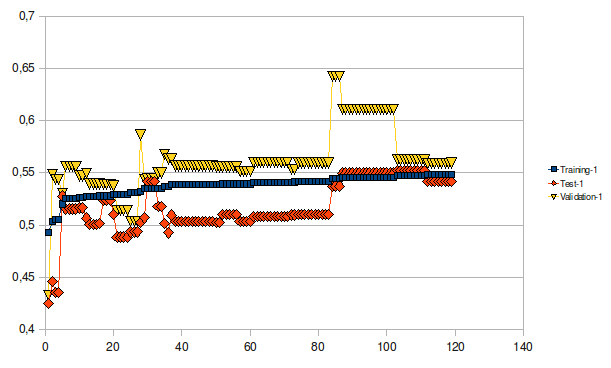
\includegraphics[scale=0.75]{pholus/pholus1.png}
\end{center}
\caption{càlcul 1}
\label{fig:pholusResult1}
\end{figure}

\begin{figure}[h]
\begin{center}
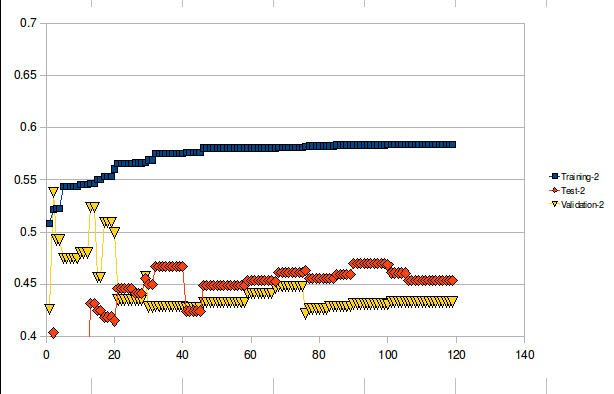
\includegraphics[scale=0.75]{pholus/pholus2.png}
\end{center}
\caption{càlcul 2}
\label{fig:pholusResult2}
\end{figure}

\begin{figure}[h]
\begin{center}
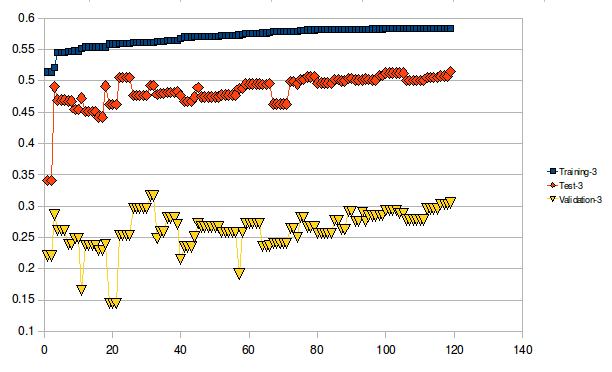
\includegraphics[scale=0.75]{pholus/pholus3.png}
\end{center}
\caption{càlcul 3}
\label{fig:pholusResult3}
\end{figure}

\begin{figure}[h]
\begin{center}
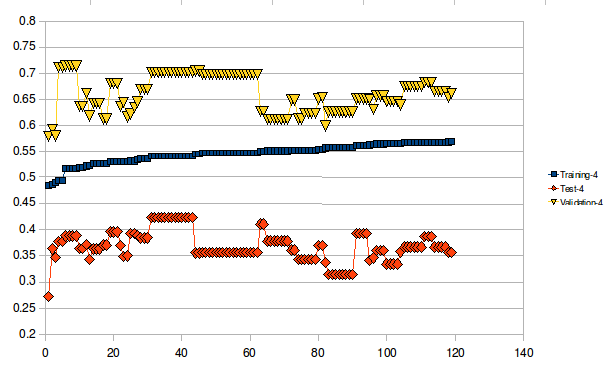
\includegraphics[scale=0.75]{pholus/pholus4.png}
\end{center}
\caption{càlcul 4}
\label{fig:pholusResult4}
\end{figure}

\begin{figure}[h]
\begin{center}
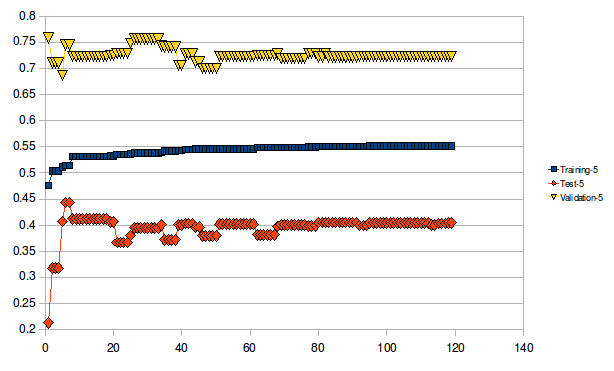
\includegraphics[scale=0.75]{pholus/pholus5.png}
\end{center}
\caption{càlcul 5}
\label{fig:pholusResult5}
\end{figure}

\begin{figure}[h]
\begin{center}
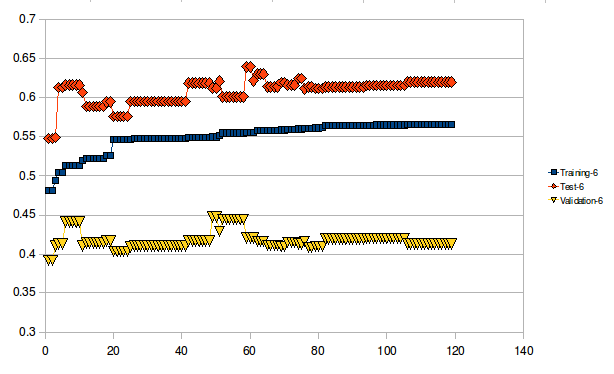
\includegraphics[scale=0.75]{pholus/pholus6.png}
\end{center}
\caption{càlcul 6}
\label{fig:pholusResult6}
\end{figure}

\begin{figure}[h]
\begin{center}
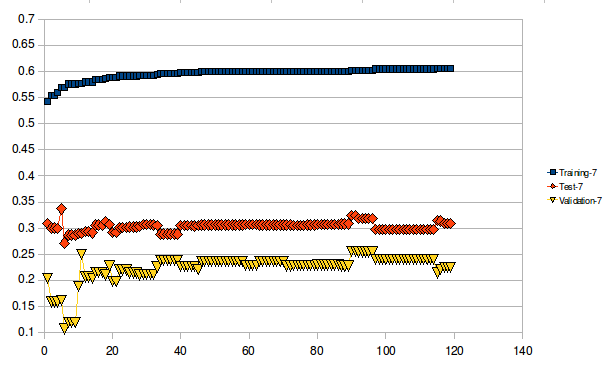
\includegraphics[scale=0.75]{pholus/pholus7.png}
\end{center}
\caption{càlcul 7}
\label{fig:pholusResult7}
\end{figure}

\begin{figure}[h]
\begin{center}
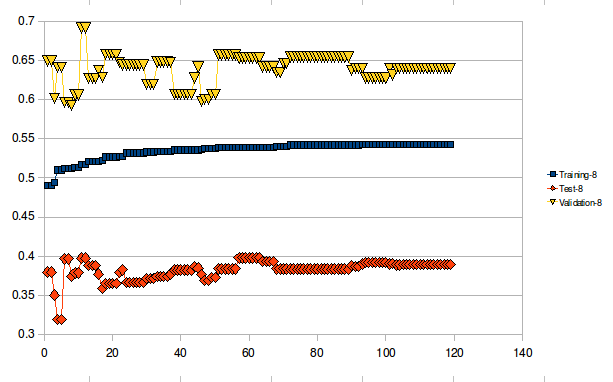
\includegraphics[scale=0.75]{pholus/pholus8.png}
\end{center}
\caption{càlcul 8}
\label{fig:pholusResult8}
\end{figure}

\begin{figure}[h]
\begin{center}
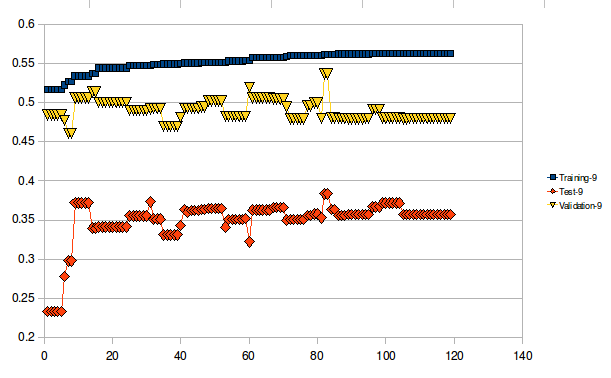
\includegraphics[scale=0.75]{pholus/pholus9.png}
\end{center}
\caption{càlcul 9}
\label{fig:pholusResult9}
\end{figure}

\begin{figure}[h]
\begin{center}
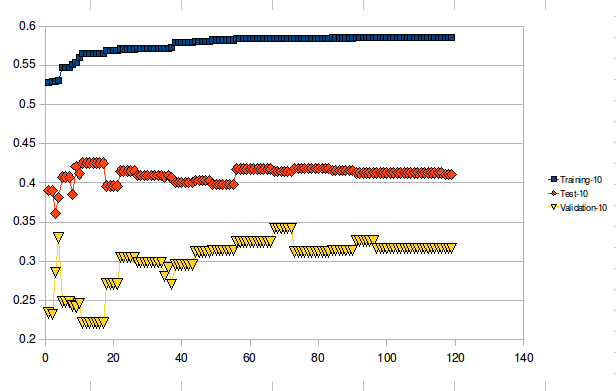
\includegraphics[scale=0.75]{pholus/pholus10.png}
\end{center}
\caption{càlcul 10}
\label{fig:pholusResult10}
\end{figure}

% subsection Anàlisi de Resultats (end)
% section Resultats (end)
\section{Conclusions i treball futur} % (fold)
\label{sec:PConclusions i treball futur}
En aquest projecte hem desenvolupat exitosament un programari que ha permès ser
més eficients en un procés que ja existia, però nosaltres l'hem millorat, no
només en sentit d'aproximació química, sinó aprofitant-nos de les aventatges que
ens ofereixen els algorismes genètics, permetent-nos explorar un espai de
possibles solucions immens, en un temps raonable (entre 2 i 8 hores segons el
tamany del problema).

La exploració d'aquest problema ens ha servit per aprendre una mica sobre
les unions entre lligands i dianes i també les maneres de agrupar molècules per
famílies, però sobretot ha servit per a provar que els algorismes genètics poden
donar solucions reals i viables a problemes que són molt difícils de solucionar
amb altres tècniques.

Pholus, però no és un projecte tancat, i de fet, ja s'ha ampliat i millorat
respecte al que es presenta aquí, amb una interfície web i un sistema de mails
per a reportar la finalització dels càlculs als usuaris.

% section Conclusions i treball futur (end)
\end{document}
